% Structure of the formalization, shown in README.md.
% Build: pdflatex proof-structure.tex, then pdftocairo -svg proof-structure.pdf proof-structure.svg.
% Mid-tone boxes with white text and mid grey arrows, so one image serves light and dark pages.
\documentclass[10pt,tikz,border=3pt]{standalone}
\usepackage[T1]{fontenc}
\usepackage[default]{sourcesans}
\usepackage[scale=0.9]{sourcecodepro}
\usepackage{amssymb}
\usetikzlibrary{arrows.meta,calc}

\definecolor{fg}{HTML}{FFFFFF}\definecolor{muted}{HTML}{E8EDF2}\definecolor{arrow}{HTML}{8C959F}
\definecolor{blueF}{HTML}{325A8C}\definecolor{blueB}{HTML}{4F79AD}\definecolor{blueL}{HTML}{BCD4F2}
\definecolor{greenF}{HTML}{2D6B49}\definecolor{greenB}{HTML}{4A8E68}\definecolor{greenL}{HTML}{B8E2C8}
\definecolor{orangeF}{HTML}{9C5622}\definecolor{orangeB}{HTML}{C27238}\definecolor{orangeL}{HTML}{F6CFA9}
\definecolor{grayF}{HTML}{4A525D}\definecolor{grayB}{HTML}{6B747F}\definecolor{grayL}{HTML}{D7DEE6}

% bar proportional to lines of code: {thousands of lines}{lines, formatted}{files}{colour}
\newcommand\codebar[4]{%
  \pgfmathsetlengthmacro\barlen{#1/66.719*2.5cm}%
  {\color{#4}\rule[-0.6pt]{\barlen}{6pt}}\hspace{5pt}{\color{muted}\footnotesize #2 lines, #3 files}}
\newcommand\cardtitle[2]{{\bfseries #1}\hfill{\color{muted}\ttfamily #2}\par\vspace{2pt}}
\newcommand\lean[1]{\mbox{\ttfamily #1}}
\newcommand\src[1]{\mbox{[#1]}}

\begin{document}
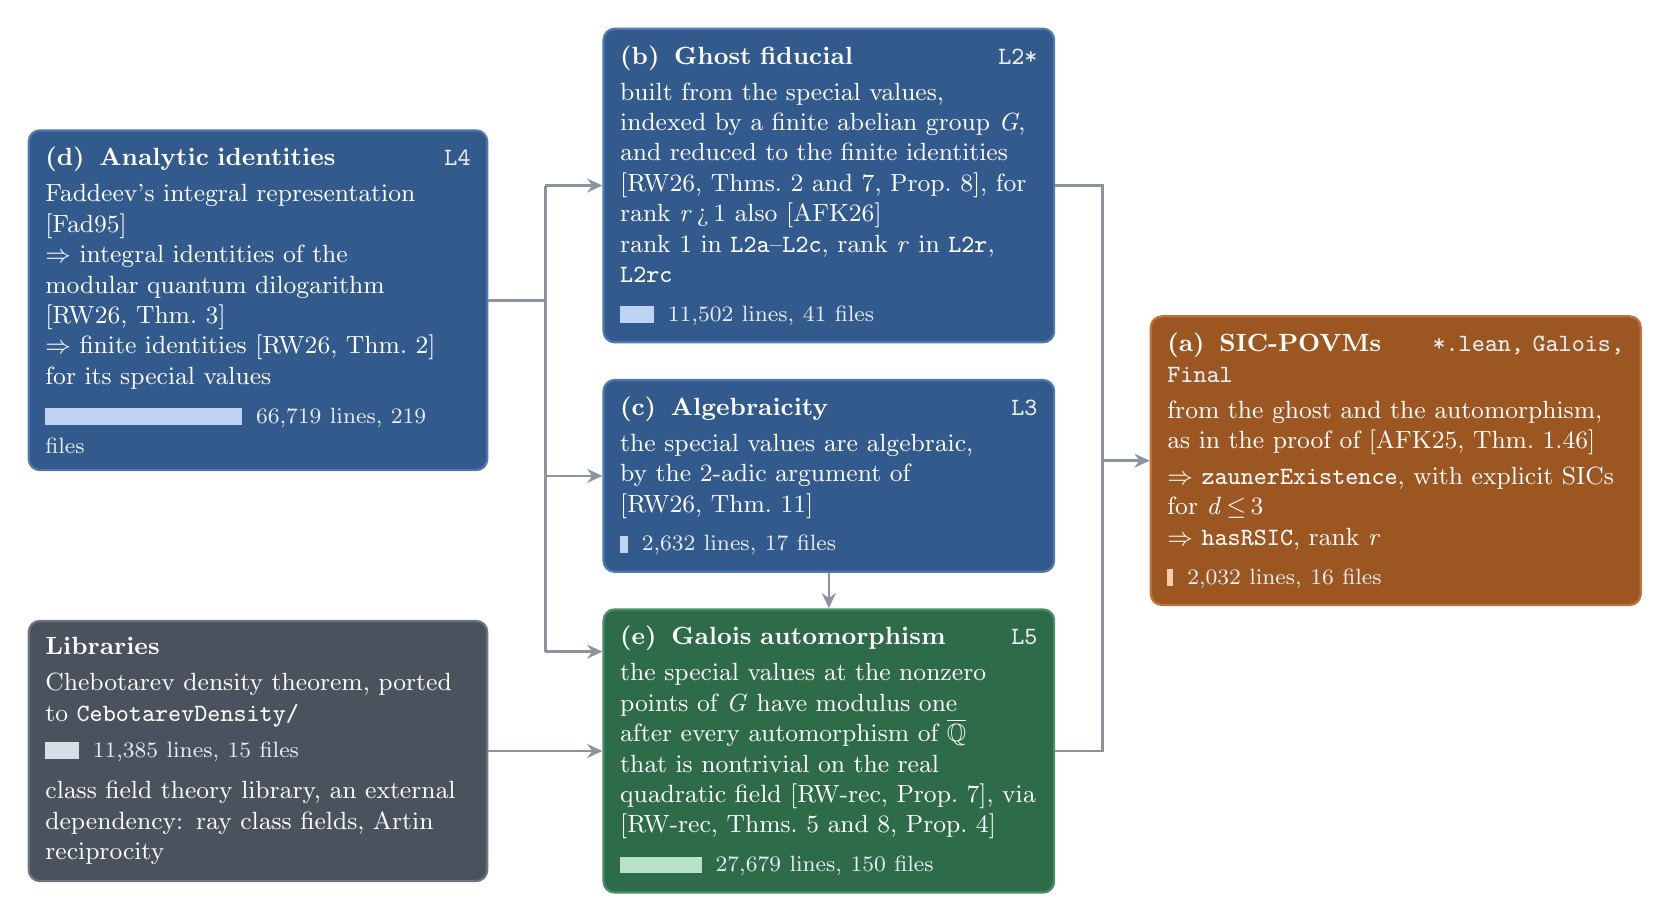
\begin{tikzpicture}[
    font=\small, text=fg,
    card/.style 2 args={draw=#1B, fill=#1F, rounded corners=4pt, line width=0.8pt,
      text width=#2, inner sep=6pt, align=left, anchor=north west,
      execute at begin node={\hyphenpenalty=10000\exhyphenpenalty=10000}},
    arr/.style={-{Stealth[length=5.5pt,width=5pt]}, line width=0.9pt, draw=arrow},
    line/.style={line width=0.9pt, draw=arrow}]

  % column 2
  \node[card={blue}{5.3cm}] (b) at (7.3,0) {%
    \cardtitle{(b)\enspace Ghost fiducial}{L2*}
    built from the special values, indexed by a finite abelian group \textit{G}, and reduced to the finite identities \src{RW26, Thms.~2 and 7, Prop.~8}, for rank \textit{r}\,>\,1 also \src{AFK26}\par
    rank 1 in \lean{L2a}--\lean{L2c}, rank \textit{r} in \lean{L2r}, \lean{L2rc}\par\vspace{3pt}
    \codebar{11.502}{11,502}{41}{blueL}};
  \node[card={blue}{5.3cm}] (c) at ($(b.south west)+(0,-0.45)$) {%
    \cardtitle{(c)\enspace Algebraicity}{L3}
    the special values are algebraic, by the 2-adic argument of \src{RW26, Thm.~11}\par\vspace{3pt}
    \codebar{2.632}{2,632}{17}{blueL}};
  \node[card={green}{5.3cm}] (e) at ($(c.south west)+(0,-0.45)$) {%
    \cardtitle{(e)\enspace Galois automorphism}{L5}
    the special values at the nonzero points of \textit{G} have modulus one after every automorphism of $\overline{\mathbb{Q}}$ that is nontrivial on the real quadratic field \src{RW-rec, Prop.~7}, via \src{RW-rec, Thms.~5 and 8, Prop.~4}\par\vspace{3pt}
    \codebar{27.679}{27,679}{150}{greenL}};

  % column 1, (d) centred on (b) and (c), libraries centred on (e)
  \path ($(b.north)!0.5!(c.south)$) coordinate (dmid);
  \node[card={blue}{5.4cm}, anchor=west] (d) at (0,0 |- dmid) {%
    \cardtitle{(d)\enspace Analytic identities}{L4}
    Faddeev's integral representation \src{Fad95}\par
    $\Rightarrow$ integral identities of the modular quantum dilogarithm \src{RW26, Thm.~3}\par
    $\Rightarrow$ finite identities \src{RW26, Thm.~2} for its special values\par\vspace{3pt}
    \codebar{66.719}{66,719}{219}{blueL}};
  \node[card={gray}{5.4cm}, anchor=west] (lib) at (0,0 |- e.west) {%
    \cardtitle{Libraries}{}
    Chebotarev density theorem, ported to \lean{CebotarevDensity/}\par\vspace{2pt}
    \codebar{11.385}{11,385}{15}{grayL}\par\vspace{4pt}
    class field theory library, an external dependency: ray class fields, Artin reciprocity};

  % column 3
  \path ($(b.north)!0.5!(e.south)$) coordinate (amid);
  \node[card={orange}{5.8cm}, anchor=west] (a) at ($(b.east |- amid)+(1.2,0)$) {%
    \cardtitle{(a)\enspace SIC-POVMs}{*.lean, Galois, Final}
    from the ghost and the automorphism, as in the proof of \src{AFK25, Thm.~1.46}\par\vspace{2pt}
    $\Rightarrow$ \lean{zaunerExistence}, with explicit SICs for \textit{d}\,$\le$\,3\par
    $\Rightarrow$ \lean{hasRSIC}, rank \textit{r}\par\vspace{3pt}
    \codebar{2.032}{2,032}{16}{orangeL}};

  % (d) feeds (b), (c), (e) through one bus
  \coordinate (busL) at ($(d.east)!0.5!(b.west |- d.east)$);
  \draw[line] (d.east) -- (busL |- d.east);
  \draw[line] (busL |- b.west) -- ($(busL |- e.north west)+(0,-0.55)$);
  \draw[arr] (busL |- b.west) -- (b.west);
  \draw[arr] (busL |- c.west) -- (c.west);
  \draw[arr] ($(busL |- e.north west)+(0,-0.55)$) -- ($(e.north west)+(0,-0.55)$);
  % libraries and algebraicity feed (e)
  \draw[arr] (lib.east |- e.west) -- (e.west);
  \draw[arr] (c.south) -- (e.north);
  % (b) and (e) feed (a)
  \coordinate (busR) at ($(b.east)!0.5!(a.west |- b.east)$);
  \draw[line] (b.east) -- (busR |- b.east) -- (busR |- e.east) -- (e.east);
  \draw[arr] (busR |- a.west) -- (a.west);

\end{tikzpicture}
\end{document}
